\documentclass[a4paper,11pt,oneside]{book}
\usepackage[T1]{fontenc}
\usepackage[utf8]{inputenc}
\usepackage{lmodern}

%%%Problem Solution Dependency%%%
\usepackage[auto-label]{exsheets}
\usepackage{hyperref}

\usepackage{mdframed}

%%%Styling%%%
\usepackage{indentfirst}


\usepackage{amsmath}
\usepackage{enumitem}

%%%Spacing%%%
\usepackage{geometry}
\usepackage[utf8]{inputenc}

%%%Multiple Choice%%%
\usepackage{multicol}

%%%Figures%%%
\usepackage{graphicx}
\graphicspath{ {./Kinematics/} }

%%%%%%%%%%%%
% PAGE ONE %
%%%%%%%%%%%%
\title{\Huge \textbf{Kinematics Tips \& Tricks} \\ \huge https://qilinxue.github.io/physics-problems/Kinematics/Standalone.pdf}
\author{\textsc{QiLin Xue}}

\begin{document}

\maketitle
\tableofcontents

\chapter{Kinematics}
(To view the full document with answers, go to https://qilinxue.github.io/physics-problems/Kinematics/Standalone.pdf)

Kinematics is the study of the motion of objects.
\\\\
In this chapter, we will be using the constants $x, v, a$ to represent position, velocity, and acceleration, respectively.  Unless otherwise stated, subscripts "$0 \; and \; f$" will be given to represent the original and final value of the variable. (e.g. $v_0$ is the starting velocity and $v_f$ is the final velocity)
\\\\
It is important to know that the problems we will be dealing with have \emph{uniform accelerated motion}, meaning the acceleration does not change.

\section{Equations}
\begin{equation}
    F=\frac{|Q_1Q_2|}{4\pi\epsilon_0R^2}
\end{equation}
\begin{equation}
    \frac{F}{Q}=\frac{F_{any\;charge}}{Q_{any\;charge}}=E
\end{equation}
\begin{equation}
    E_{net}=E_1+E_2+E_3+\dots+E_N
\end{equation}
\begin{equation}
    V=\frac{U}{Q} \iff
    \Delta V=\frac{\Delta U}{Q}
\end{equation}

Many textbooks will make the substitution for coulomb's constant: $k=\frac{1}{4\pi\epsilon_0}$ to simplify Coulomb's Law (2.1) However, it is generally preferred to keep it in the long form as the $\pi$ may cancel out with other terms.

\subsection*{Calculus}

The only calculus equation needed is a direct restatement of (2.4). Although it has an extremely trivial derivation for any calculus student, it is vital in solving many problems involving calculus.

\begin{equation}
    E_x=-\frac{dV}{dx}
\end{equation}

\section{Tricks}
\subsection{General Steps}
The most difficult part about kinematics is collecting the information, and interpreting the question correctly. Here are the general steps to solve any kinematic problem:
\begin{enumerate}
  \item List down all the variables you are given, and their respective values. 
  \item Determine and list the unknown variable you want to solve for.
  \item Track down the appropriate equation that involves only the variables you listed above.
  \item Substitute in the values, and solve for the unknown.
  \item Double check your work. Do an unit analysis and check if it makes sense.
\end{enumerate}

\subsection{Free-Fall Problems}
One of the most common types of kinematic problems involve objects falling only under the force of gravity (air resistance ignored), such that their acceleration is g. The following tricks are useful in solving this type of problem:
\begin{itemize}
    \item At the peak of any trajectory, the object's y-component of velocity is zero. This is often used to calculate the peak height (by setting the velocity equal to zero).
    \item Because of conservation of energy, and as reflected mathematically in the symmetry of parabolas, an object's \emph{speed} as it passes a certain height is exactly the same on the way up as it is on the way down.
    \item Also because of the symmetry of parabolas, the magnitude of the time difference between when the object is at the peak of its trajectory ($t_{peak}$) and when it is at a particularly y-position below its peak is the same whether the object is ascending or descending at the latter position.
    \item You should memorize $g = 9.8\frac{m}{s^2}$ however for the purposes of this guide, you can use $g = 10\frac{m}{s^2}$. You can set g to be negative or positive, as long as you keep your positive direction constant throughout each question!
\end{itemize}

\newpage
\section{Problems}
\SetupExSheets{
  question/post-body-hook = {%
    \hyperlink{sol:\CurrentQuestionID}{ (View Solution)}
  },
  solution/pre-hook = {
    \hypertarget{sol:\CurrentQuestionID}{}%
  } ,
  solution/pre-body-hook = {%
    \hyperref[qu:\CurrentQuestionID]{ (View Question)}\par
  }
}

\SetupExSheets{
  counter-format = ch.3.qu,
  headings=runin
} 

\subsection*{Regular}
%%%%%%%%%%%%%%%%%%%%%%%%%%%%%%%%%%
%%%%%%%%%%%%%%%%%%%%%%%%%%%%%%%%%%
%%%%%%%%%%%%%%%%%%%%%%%%%%%%%%%%%%

\begin{question}
What are the units for permittivity of free space $\epsilon_0$?

\end{question}

\begin{solution}

Rearrange the equation to solve for $\epsilon_0$, and give all variables a value of 1 in order to figure out the units for $\epsilon_0$. Please note, that we are giving everything a value of 1 for the sole purpose of making adding, multiplying, and dividing units much easier. It of course is not necessary, but helps to build an intuition of dimensional analysis.

The final value of course, is going to be incorrect, but we only care about the units. Because of this, we can ignore $2\pi$ since it is dimensionless.

\begin{equation*}
F = \frac{Q_1Q_2}{\epsilon_0R^2} \rightarrow
\epsilon_0 = \frac{Q_1Q_2}{FR^2} \rightarrow
\epsilon_0 = \frac{(1C)(1C)}{(1N)(1m)^2} \rightarrow
\epsilon_0 = (1C^2)(1N^{-1})(1m^{-2})
\end{equation*}

Thus $\epsilon_0$ has SI units of $C^2N^{-1}m^{-2}$
\end{solution}

%%%%%%%%%%%%%%%%%%%%%%%%%%%%%%%%%%
%%%%%%%%%%%%%%%%%%%%%%%%%%%%%%%%%%
%%%%%%%%%%%%%%%%%%%%%%%%%%%%%%%%%%

\begin{question}
Two $1\mu C$ charges lie at (1,0) and at (0,1).
\begin{enumerate}[label=(\alph*)]
    \item Calculate the magnitude of the force that $1-\mu C$ charge at (0,1) exerts on the $1\mu C$ charge at (1,0)
    \item Calculate the components of this force in the x- and y-directions and express the force as a vector.
\end{enumerate}
\end{question}

\begin{solution}

The first thing we do is draw a diagram: see the figure below. We are attempting to calculate the force, and since the charges of both particles are already given to us, we need to figure out the distance separating them which can be done using geometry.

\begin{center}
% \begin{tikzpicture}
% \begin{axis}[
%     axis lines=middle,
%     xmin=0, xmax=2,
%     ymin=0, ymax=2,
%     xtick=1, ytick=1,
%     xlabel = $x$,
%     ylabel = $y$,
% ]
% \addplot [only marks] table {
% 1   0
% 0   1
% };

% \addplot [domain=-10:10, samples=2, dashed] {1-x};
% \end{axis}
% \end{tikzpicture}
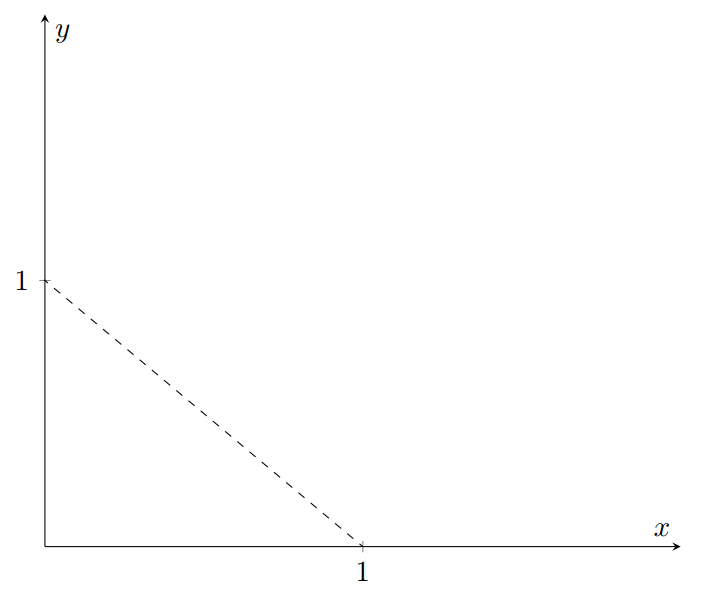
\includegraphics[scale=0.9]{Figures/Figure26}
\end{center}
(A) Thus the force is, using (2.1):
\begin{equation*}
    F=\frac{Q_1Q_2}{2\pi\epsilon_0R^2}=
    \frac{(1 \times 10^{-6}C)^2}
    {(2\pi)(8.854 \times 10^{-12}C^2N^{-1}m^{-2})(\sqrt{1^2 + 1^2}^2)}
\end{equation*}
\begin{equation*}
    F = 4.5 \times 10^{-3} N
\end{equation*}

(B) To calculate the components, we break up the \emph{magnitude} of the force we calculated in part A into components using standard geometry. Note that the y component is negative, because the charge at (1,0) will be wanting to move in the negative y and positive x direction.
\begin{equation*}
    \left\{
        \begin{array}{ll}
            F_x = (4.5 \times 10^{-3} N)cos(45^\circ) = 3.18 \times 10^{-3} N
            \\
            F_y = -(4.5 \times 10^{-3} N)cos(45^\circ) = -3.18 \times 10^{-3} N
        \end{array}
              \right.
\end{equation*}

Combining everything together gives the force vector:

\begin{equation*}
    \vec{F} = (3.18 \times 10^{-3} N)\hat{i} - 
              (3.18 \times 10^{-3} N)\hat{j}    
\end{equation*}

\end{solution}

%%%%%%%%%%%%%%%%%%%%%%%%%%%%%%%%%%
%%%%%%%%%%%%%%%%%%%%%%%%%%%%%%%%%%
%%%%%%%%%%%%%%%%%%%%%%%%%%%%%%%%%%

\begin{question}
A point charge +Q is located at the origin and a point charge -2Q is located at (1,0). Where is the electric field equal to zero? (Everything is in SI units)

\end{question}

\begin{solution}
The first thing to realize is that the only place the electric field can ever be zero is along the x-axis.\footnote{think about suspending an object under two magnets. It only works if it's directly underneath both of them!} Before we brute force, let's make a diagram and think about the question qualitatively.

% \begin{center}
%   \begin{tikzpicture}[scale=2]
%     \draw (-3,0) -- (3,0);
%     \foreach \i in {-3,-2,...,3} % numbers on line
%       \draw (\i,0.1) -- + (0,-0.2) node[below] {$\i$};
%     \fill[blue] (0,0) circle (0.5 mm);
%     \fill[red]  (1,0) circle (1 mm);
%   \end{tikzpicture}   
% \end{center}
\begin{center}
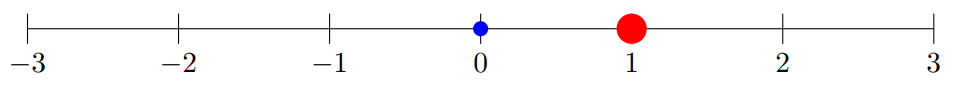
\includegraphics{Figures/Figure27}
\end{center}
Where on the x-axis should we look for solutions? We have three options:
\begin{enumerate}
    \item Between (0,0) and (1,0): both charges produce an electric field in the +x direction.
    \item Between (1,0) and $\infty$: In this region, the -2Q charge is always dominant, also providing a nonzero electric field.
    \item Between (0,0) and -$\infty$: In this region, when we are very close to the +Q charge, the +Q charge will dominate. However, as we move further and further away, the effects of distance will be less and less prominent and the -2Q charge will come to dominate. We will call this location (x,0)
\end{enumerate}
 
To do the math, we simply need to use superposition:

\begin{equation}
    E_{net} = E_{+Q} + E_{-2Q} \rightarrow
    0 = \frac{Q}{4\pi\epsilon_0x^2} + 
        \frac{-2Q}{4\pi\epsilon_0(1-x)^2}
\end{equation}
\begin{equation}
    \frac{Q}{4\pi\epsilon_0x^2} = 
    \frac{2Q}{4\pi\epsilon_0(1-x)^2} \rightarrow
    \frac{1}{x^2} = \frac{2}{(1-x)^2} \rightarrow
    2x^2 = (x+1)^2
\end{equation}

Solving this quadratic relation gives $x=-1\pm\sqrt{2}$. Since we already established that x is negative, we know the electric field is zero at $x=-1-\sqrt{2}$

\end{solution}

%%%%%%%%%%%%%%%%%%%%%%%%%%%%%%%%%%
%%%%%%%%%%%%%%%%%%%%%%%%%%%%%%%%%%
%%%%%%%%%%%%%%%%%%%%%%%%%%%%%%%%%%

\begin{question}
A point charge $Q_1$ is located at the origin and a point charge $Q_2$ is located at (5,0). Which of the following situations have a point or points where the potential is zero? (more than one may apply)

\begin{center}
\begin{tabular}{ |c|c|c| } 
 \hline
       & $Q_1$ & $Q_2$ \\ 
 I      & +q  & +3q  \\ 
 II     & -q  & +17q \\ 
 III    & -3q & -q   \\ 
 \hline
\end{tabular}
\end{center}

\end{question}


\begin{solution}
Using the superposition formula for potential, we see that it is only possible for potential to be zero, when the charges have opposite signs:

\begin{equation*}
    V_{net}=0=\frac{Q_1}{x^2}+\frac{Q_2}{(5-x)^2}
\end{equation*}

Therefore, II is the correct answer.

Another solution is to draw the graphs of V(x) for each individual charge, and then superposition them like in the following figure:

\begin{center}
% \begin{tikzpicture}
% \begin{axis}[
%     axis lines=middle,
%     xmin=-20, xmax=20,
%     ymin=-20, ymax=20,
%     xlabel = $x$,
%     ylabel = $V$,
% ]
% %Below the red is defined
% \addplot [
%     domain=-20:20, 
%     samples=100, 
%     color=red,
%     style={ultra thick}
% ]
% {-1/(x^2)};
% \addlegendentry{$V_{-q}$}

% %Here the blue is defined
% \addplot [
%     domain=-20:20, 
%     samples=100, 
%     color=blue,
%     style={ultra thick},
% ]
% {17*x/((6-x)^2)};
% \addlegendentry{$V_{17q}$}

% \end{axis}
% \end{tikzpicture}
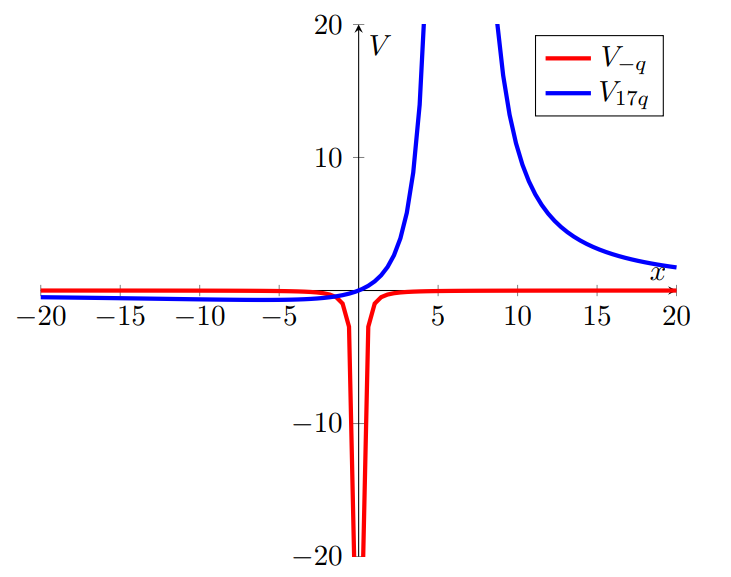
\includegraphics{Figures/Figure28}
\end{center}

All we need to prove is that if we add these two functions, it will have at least one real root. This proof will be left as an exercise to the reader.\footnote{Hint: You can prove this in two ways. Either use the mean value theorem, or notice that the peaks and troughs are located at different locations...}

\end{solution}

%%%%%%%%%%%%%%%%%%%%%%%%%%%%%%%%%%
%%%%%%%%%%%%%%%%%%%%%%%%%%%%%%%%%%
%%%%%%%%%%%%%%%%%%%%%%%%%%%%%%%%%%

\begin{question}
Which of the three charge distributions introduced in the previous exercise has point(s) where the electric field is zero?
\end{question}

\begin{solution}
We have already proved in an earlier exercise that in, the electric field between two opposite charges different in magnitude, there is one point where it is zero. In a charge distribution where both charges have equal signs, there is also one place where the electric field is zero, this time in between both charges. This is the spot where the charges cancel out.

The answer is I,II and III
\end{solution}

%%%%%%%%%%%%%%%%%%%%%%%%%%%%%%%%%%
%%%%%%%%%%%%%%%%%%%%%%%%%%%%%%%%%%
%%%%%%%%%%%%%%%%%%%%%%%%%%%%%%%%%%

\begin{question}
Points $Q_1$, $Q_2$, $Q_3$, and $Q_4$ are located at (-1,1),(1,1),(1,-1),(-1,-1) respectively. Which of the following charge distributions is the electric field zero at the origin?

\begin{center}
\begin{tabular}{ |c|c|c|c|c| } 
 \hline
       & $Q_1$ & $Q_2$ & $Q_3$ & $Q_4$ \\ 
 I        & +q  & +q & -q & -q  \\ 
 II       & +q  & -q & +q & -q  \\ 
 III      & +q  & -q & +q & +q  \\ 
 IV       & +q  & +q & +q & +q  \\ 
 V        & -q  & -q & -q & -q  \\ 
 \hline
\end{tabular}
\end{center}

\end{question}

\clearpage
\begin{solution}
The table is too confusing, so let's graph out $Q_1$, $Q_2$, $Q_3$, and $Q_4$ on a square:

\begin{center}
% \begin{tikzpicture}
% \draw (0,0) -- (0,2) -- (2,2) -- (2,0) -- (0,0);
% \node[above right] at (0,0) {$Q_4$};
% \node[below right] at (0,2) {$Q_1$};
% \node[below left] at (2,2) {$Q_2$};
% \node[above left] at (2,0) {$Q_3$};
% \end{tikzpicture}
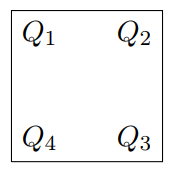
\includegraphics{Figures/Figure29}
\end{center}

In order for the center of the square to have a zero electric field, the electric field must be zero when the point charges are superimposed. We can superimpose the charges diagonally. This is possible if and only if $Q_1 = Q_3$ and $Q_2 = Q_4$ only II,IV,V satisfy this criteria.

\end{solution}

%%%%%%%%%%%%%%%%%%%%%%%%%%%%%%%%%%
%%%%%%%%%%%%%%%%%%%%%%%%%%%%%%%%%%
%%%%%%%%%%%%%%%%%%%%%%%%%%%%%%%%%%

\begin{question}
Which of the charge distributions introduced in the previous question is the potential zero at the origin?
\end{question}

\begin{solution}
The potential is zero at the origin if and only if the superposition of potential is equal to zero. Since potential is a scaler and all the charges are equidistant from the origin, this means that the total net charge at the origin has to be zero. In other words, the potential is zero, if and only if:

\begin{equation*}
    Q_1+Q_2+Q_3+Q_4=0
\end{equation*}

Only I, and II satisfy this criteria.

\end{solution}

%%%%%%%%%%%%%%%%%%%%%%%%%%%%%%%%%%
%%%%%%%%%%%%%%%%%%%%%%%%%%%%%%%%%%
%%%%%%%%%%%%%%%%%%%%%%%%%%%%%%%%%%

\begin{question}
Two positive charges +Q are located on the -axis at (0,a) and (0,-a), and a third charge -q is on the positive x-axis at (x,0). Find the electric field along the x-axis as a function of position E(x), due to the positive charges.
\end{question}

\begin{solution}
First, calculate the magnitude of the electric field as a function of position. Use the electric field equation (directly derived from Coulomb's Law) to figure out the electric field from one charge:

\begin{equation*}
    |E(x)| = \frac{Q}{4\pi\epsilon_0\sqrt{(x^2+a^2)}^2} =
             \frac{Q}{4\pi\epsilon_0(x^2+a^2)}
\end{equation*}

Now, to separate the magnitude of the electric field along the x-axis, using standard trigonometry techniques:

\begin{equation*}
    E(x)_x = |E(x)|cos(\theta) = |E(x)|(\frac{x}{\sqrt{(x^2+a^2)}})
    =
    \frac{Q}{4\pi\epsilon_0(x^2+a^2)}(\frac{x}{\sqrt{(x^2+a^2)}})
\end{equation*}

\begin{equation*}
    E(x)_x =
    \frac{Qx}{4\pi\epsilon_0(x^2+a^2)^{3/2}}
\end{equation*}

However, since we have two equally charged particles on the y-axis, we can superimpose them to get the final answer.\footnote{Because of symmetry, we can just multiply by two, instead of doing everything all over again}

\begin{equation*}
    E(x)_x =
    \frac{2Qx}{4\pi\epsilon_0(x^2+a^2)^{3/2}} =
    \frac{Qx}{2\pi\epsilon_0(x^2+a^2)^{3/2}}
\end{equation*}

\end{solution}

%%%%%%%%%%%%%%%%%%%%%%%%%%%%%%%%%%
%%%%%%%%%%%%%%%%%%%%%%%%%%%%%%%%%%
%%%%%%%%%%%%%%%%%%%%%%%%%%%%%%%%%%

\begin{question}
Two point charges +Q are located on the x-axis at (-d,0) and (d,0). Sketch the electric field $E(x)$ along the x-axis as a function of position.
\end{question}

\begin{solution}
First, graph the individual electric fields each charge produces, then sum it up. Please note we are NOT graphing $\frac{Q}{r\pi\epsilon_0x^2}$. That gives the magnitude of the electric field. Since electric field is a vector, anything that is to the left (negative x direction) of the charge will have a negative electric field.

The individual electric fields will look like:\footnote{Because of program graphing issues, the vertical asymptotes are shown, but in reality both ends should extend to $\pm \infty$ meaning these vertical lines are not \emph{real}}

\begin{center}
% \begin{tikzpicture}
% \begin{axis}[
%     axis lines=middle,
%     xmin=-10, xmax=10,
%     ymin=-10, ymax=10,
%     xlabel = $x$,
%     ylabel = $E$,
% ]
% %Below the red is defined
% \addplot [
%     domain=-10:10, 
%     samples=100, 
%     color=red,
%     style={ultra thick}
% ]
% {1/(x-3)};
% \addlegendentry{$E(x)_{Q1}$}

% %Here the blue is defined
% \addplot [
%     domain=-10:10, 
%     samples=100, 
%     color=blue,
%     style={ultra thick},
% ]
% {1/(x+3)};
% \addlegendentry{$E(x)_{Q2}$}

% \end{axis}
% \end{tikzpicture}
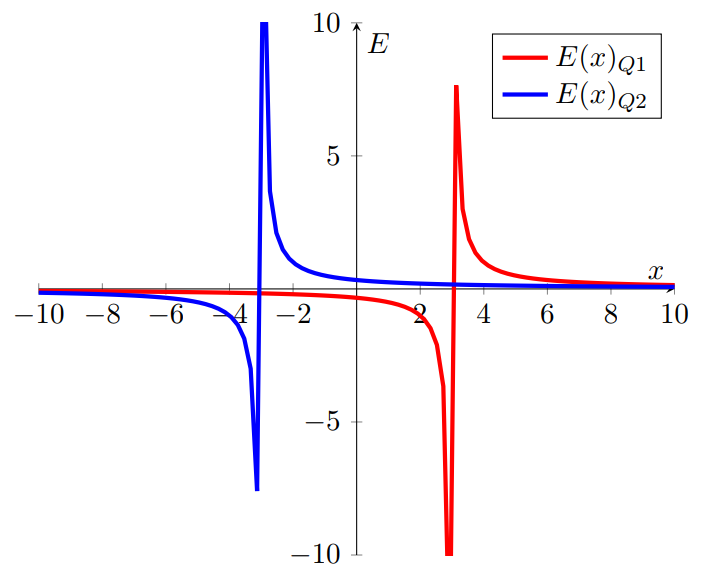
\includegraphics{Figures/Figure210}
\end{center}

And after they are superimposed, and added, it will look like:

\begin{center}
% \begin{tikzpicture}
% \begin{axis}[
%     axis lines=middle,
%     xmin=-10, xmax=10,
%     ymin=-10, ymax=10,
%     xlabel = $x$,
%     ylabel = $E$,
% ]

% %Here the purple is defined
% \addplot [
%     domain=-10:10, 
%     samples=100, 
%     color=purple,
%     style={ultra thick},
% ]
% {(1/(x+3))+(1/(x-3))};

% \end{axis}
% \end{tikzpicture}
% 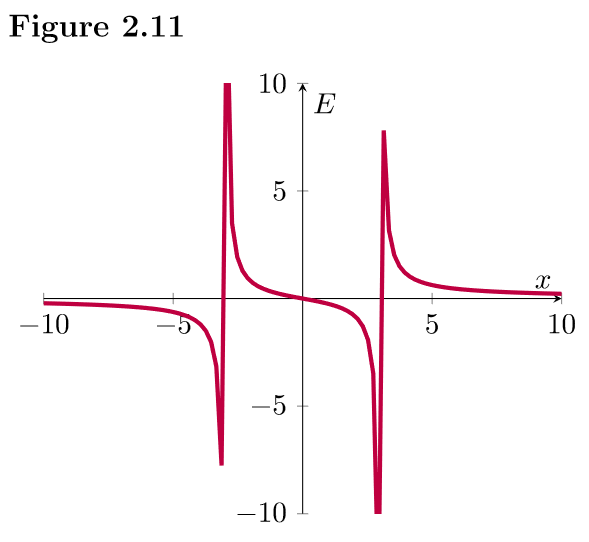
\includegraphics{Figures/Figure211}
TBA
\end{center}

\end{solution}


%%%%%%%%%%%%%%%%%%%%%%%%%%%%%%%%%%
%%%%%%%%%%%%%%%%%%%%%%%%%%%%%%%%%%
%%%%%%%%%%%%%%%%%%%%%%%%%%%%%%%%%%

\subsection*{Calculus}

\begin{question}
A charge of -Q is located at the origin, and two charges of +Q are located along the y-axis at (0,-a) and (0,a).

\begin{enumerate}[label=(\alph*)]
    \item Calculate the electric field along the x-axis, E(x)
    \item Calculate the approximate form of E(x) for very small x.
    \item Calculate the approximate form of E(x) for very large x.
\end{enumerate}
\end{question}

\begin{solution}

(A) Along the +x axis, symmetry dicates that the field must point in the x-direction. Summing the contributions of the x-components of the electric fields due to the three point charges yields the following (The vector geometry is the same as one of the previous questions. If you haven't done them, do them now!)

\begin{equation*}
    E_{net} = E_{-Q} + 2E_{+Q} \rightarrow
    E_{net} = \frac{-Q}{4\pi\epsilon_0x^2}
              +2[\frac{Q}{4\pi\epsilon_0(x^2+a^2)}
                 \frac{x}{\sqrt{x^2+a^2}}]
\end{equation*}
\begin{equation*}
    E_{net} = \frac{-Q}{4\pi\epsilon_0x^2} +
              \frac{Qx}{4\pi\epsilon_0(x^2+a^2)^{3/2}}
\end{equation*}

(B) To approximate for very small x, we will make the following approximation:

\begin{equation*}
    x^2+a^2\approx a^2
\end{equation*}

Therefore:

\begin{equation*}
    E_{net} = \frac{-Q}{4\pi\epsilon_0x^2} +
              \frac{Qx}{4\pi\epsilon_0(x^2+a^2)^{3/2}}
            \approx
            \frac{-Q}{4\pi\epsilon_0x^2} +
              \frac{Qx}{4\pi\epsilon_0 a^3}
\end{equation*}

But since:

\begin{equation*}
    \frac{1}{x^2} \gg x
\end{equation*}

Then:

\begin{equation*}
    E_{net} \approx 
                \frac{-Q}{4\pi\epsilon_0x^2} +
                \frac{Qx}{4\pi\epsilon_0 a^3}
            \approx
                \frac{-Q}{4\pi\epsilon_0x^2}
\end{equation*}

(C) To approximate for very large x, we can make a similar approximation:

\begin{equation*}
    x^2+a^2 \approx x^2
\end{equation*}

Therefore:

\begin{equation*}
    E_{net} = \frac{-Q}{4\pi\epsilon_0x^2} +
              \frac{Qx}{4\pi\epsilon_0(x^2+a^2)^{3/2}}
            \approx
              \frac{-Q}{4\pi\epsilon_0x^2} +
              \frac{Qx}{4\pi\epsilon_0x^3}
            =
              \frac{Q}{4\pi\epsilon_0x^2}
\end{equation*}

If you're not illiterate, you would have realized this is just the standard electric field equation! This is because when you are \emph{very} far away from the origin, it's impossible to see the separation of the three charges, it seems that they're all at the origin. The resulting field is due to the sum of the three charges: $Q_{effective}=Q+Q-Q=Q$, at the origin

\end{solution}

%%%%%%%%%%%%%%%%%%

\begin{question}
Consider the potential-vs-position function shown in the figure below. At which of the following points does a charge feel the greatest force in the +x direction?

\begin{center}
% \begin{tikzpicture}[scale=0.95]
% \begin{axis}[
%     axis lines=middle,
%     xmin=-4, xmax=4,
%     ymin=-2, ymax=1,
%     xlabel = $x$,
%     ylabel = $V$,
% ]
% %Below the red is defined
% \addplot [
%     domain=-10:10, 
%     samples=100, 
%     color=red,
%     style={ultra thick}
% ]
% {-2^(-x^2)};
% \addlegendentry{$V(x)$}

% \end{axis}
% \end{tikzpicture}
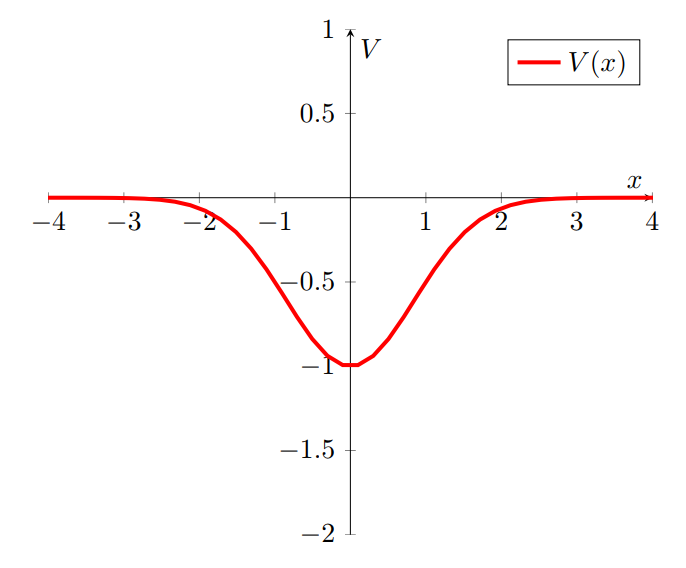
\includegraphics[scale=0.8]{Figures/Figure23}
\end{center}
\begin{multicols}{5}
\begin{enumerate}[label=(\alph*)]
    \item x=-4
    \item x=-1
    \item x=0
    \item x=1
    \item x=4
\end{enumerate}
\end{multicols}
\end{question}

\begin{solution}

Recall that the electric field is the negative slope of the potential curve: $E_x=-\frac{dV}{dx}$ so the place where the force when the slope of the potential curve has a negative value with the greatest magnitude, which is at x=-1.
\end{solution}

%%%%%%%%%%%%%%%%%%%%%%%%%%%%%%%%%%%%%%%%%%%%%%%%%%%%%%%%%%%%%%%%

\SetupExSheets{
  solution/pre-body-hook = {%
    \hyperref[qu:\CurrentQuestionID]{ (View Question)}
  }
}

%%%%%%%%%%%%%%%%%%%%%%%%%%%%%%%%%%%%%%%%%%%%%%%%%%%%%%%%%%%%%%%%

\newpage
\subsection*{Exercises}
Only answers and hints will be provided to these exercises, with no full solution. Good luck!

%%%%%%%%%%%%%%%%%%%%%%%%%%%%%%%%%%
%%%%%%%%%%%%%%%%%%%%%%%%%%%%%%%%%%
%%%%%%%%%%%%%%%%%%%%%%%%%%%%%%%%%%

\begin{question}
(AP) A conducting sphere with a radius of 0.10 meter has $1.0 \times 10^{-9}$ coulomb of charge deposited on it. the electric field just outside the surface of the sphere is:
\begin{multicols}{5}
\begin{enumerate}[label=(\alph*)]
    \item zero
    \item $450 \frac{V}{m}$
    \item $900 \frac{V}{m}$
    \item $900 \frac{V}{m}$
    \item $4500 \frac{V}{m}$
\end{enumerate}
\end{multicols}

\end{question}

\begin{solution}
C (Hint: Just like gravitation, pretend all the charge acts from the center)
\end{solution}

%%%%%%%%%%%%%%%%%%%%%%%%%%%%%%%%%%
%%%%%%%%%%%%%%%%%%%%%%%%%%%%%%%%%%
%%%%%%%%%%%%%%%%%%%%%%%%%%%%%%%%%%

\begin{question}
(AP) A positive charge +Q located at the origin produces an electric field E at point P located at (1,0). A negative charge -2Q is placed at such a point as to produce a net field of zero at point P. The second charge will be placed on the:
\begin{enumerate}[label=(\alph*)]
    \item x-axis where x > 1
    \item x-axis where 0 < x < 1
    \item x-axis where x < 0
    \item y-axis where y > 0
    \item y-axis where y < 0
\end{enumerate}

\end{question}

\begin{solution}
C (Hint: The charges have opposite signs!)
\end{solution}

%%%%%%%%%%%%%%%%%%%%%%%%%%%%%%%%%%
%%%%%%%%%%%%%%%%%%%%%%%%%%%%%%%%%%
%%%%%%%%%%%%%%%%%%%%%%%%%%%%%%%%%%

\begin{question}
(AP) Two positive charges of magnitude q are each a distance d from the origin A of a coordinate system. At which of the following points is the electric field least in magnitude?
\begin{multicols}{5}
\begin{enumerate}[label=(\alph*)]
    \item x = -d
    \item x = 0
    \item C = d
    \item D = 2d
    \item E = 3d
\end{enumerate}
\end{multicols}

\end{question}

\begin{solution}
A (Hint: Pretend it's two magnets)
\end{solution}

%%%%%%%%%%%%%%%%%%%%%%%%%%%%%%%%%%
%%%%%%%%%%%%%%%%%%%%%%%%%%%%%%%%%%
%%%%%%%%%%%%%%%%%%%%%%%%%%%%%%%%%%

\begin{question}
(AP) Two identical conducting spheres are charged to +2Q and -Q respectively, and are separated by a distance d (much greater than the radii of the spheres). The magnitude of the force of attraction of the left sphere is $F_1$. After the two spheres are made to touch and then are re-separated by distance d the magnitude of the force on the left sphere is $F_2$. Which of the following relations are true?
\begin{multicols}{5}
\begin{enumerate}[label=(\alph*)]
    \item $2F_1=F_2$
    \item $F_1=F_2$
    \item $F_1=2F_2$
    \item $F_1=4F_2$
    \item $F_1=8F_2$
\end{enumerate}
\end{multicols}

\end{question}

\begin{solution}
E (Hint: What are their charges after they touch each other?)
\end{solution}

%%%%%%%%%%%%%%%%%%%%%%%%%%%%%%%%%%
%%%%%%%%%%%%%%%%%%%%%%%%%%%%%%%%%%
%%%%%%%%%%%%%%%%%%%%%%%%%%%%%%%%%%

\begin{question}
(AP) A rigid insulated rod, with a charge of -2Q at the top and a charge of +Q at the bottom, is placed in a uniform electric field E. The rod experiences a
\begin{enumerate}[label=(\alph*)]
    \item net force to the left and a clockwise rotation
    \item net force to the left and a counterclockwise rotation
    \item net force to the right and a clockwise rotation
    \item net force to the right and a counterclockwise rotation
    \item rotation, but no net force
\end{enumerate}
\end{question}

\begin{solution}
B (Hint: in an electric field, the positive moves to the negative...)
\end{solution}

%%%%%%%%%%%%%%%%%%%%%%%%%%%%%%%%%%
%%%%%%%%%%%%%%%%%%%%%%%%%%%%%%%%%%
%%%%%%%%%%%%%%%%%%%%%%%%%%%%%%%%%%

\begin{question}
(AP) Two small spheres have equal charges q and are separated by a distance d. The force exerted on each sphere by the other has magnitude F. If the charge on each sphere is doubled and d is halved, the force on each sphere has magnitude
\begin{multicols}{5}
\begin{enumerate}[label=(\alph*)]
    \item F
    \item 2F
    \item 4F
    \item 8F
    \item 16F
\end{enumerate}
\end{multicols}

\end{question}

\begin{solution}
E (Hint: Force is proportional to $\frac{q^2}{d^2}$)
\end{solution}

%%%%%%%%%%%%%%%%%%%%%%%%%%%%%%%%%%
%%%%%%%%%%%%%%%%%%%%%%%%%%%%%%%%%%
%%%%%%%%%%%%%%%%%%%%%%%%%%%%%%%%%%

\begin{question}
(AP) A charged particle traveling with a velocity $v$ in an electric field $E$ experiences a force $F$ that must be
\begin{enumerate}[label=(\alph*)]
    \item parallel to $v$
    \item perpendicular to $v$
    \item parallel to $v \times E$
    \item parallel to $E$
    \item perpendicular to $E$
\end{enumerate}

\end{question}

\begin{solution}
E (Hint: Check out the tricks section!)
\end{solution}

%%%%%%%%

\begin{question}
(AP) A conducting sphere of radius R carries a charge Q.  Another conducting sphere has a radius R/2, but carries the same charge.  The spheres are far apart.  The ratio of the electric field near the surface of the smaller sphere to the field near the surface of the larger sphere is most nearly

\begin{multicols}{5}
\begin{enumerate}[label=(\alph*)]
    \item 1/4
    \item 1/2
    \item 1
    \item 2
    \item 4
\end{enumerate}
\end{multicols}

\end{question}

\begin{solution}
E (Hint: Use Coulomb's Law!)
\end{solution}

%%%%%%%%%%%%%%%%%%%%%%%%%%%%%%%%%%
%%%%%%%%%%%%%%%%%%%%%%%%%%%%%%%%%%
%%%%%%%%%%%%%%%%%%%%%%%%%%%%%%%%%%
\newpage
Relate to the following configurations of electric charges located at the vertices of an equilateral triangle. Use this for the next three questions:

% \begin{tikzpicture}
% \draw (0,0) -- (2,0) -- (1,1.732) -- (0,0);
% \node[below left] at (0,0) {$+q$};
% \node[below right] at (2,0) {$+q$};
% \node[above] at (1,1.732) {$+q$};
% \node[below] at (1,1) {A};

% \draw (4,0) -- (6,0) -- (5,1.732) -- (4,0);
% \node[below left] at (4,0) {$+q$};
% \node[below right] at (6,0) {$+q$};
% \node[above] at (5,1.732) {$-q$};
% \node[below] at (5,1) {B};

% \draw (8,0) -- (10,0) -- (9,1.732) -- (8,0);
% \node[below left] at (8,0) {$-q$};
% \node[below right] at (10,0) {$-q$};
% \node[above] at (9,1.732) {$+q$};
% \node[below] at (9,1) {C};

% \end{tikzpicture}

% \begin{tikzpicture}
% \draw (0,0) -- (2,0) -- (1,1.732) -- (0,0);
% \node[below left] at (0,0) {$+q$};
% \node[below right] at (2,0) {$-q$};
% \node[above] at (1,1.732) {$-2q$};
% \node[below] at (1,1) {D};

% \draw (4,0) -- (6,0) -- (5,1.732) -- (4,0);
% \node[below left] at (4,0) {$+3q$};
% \node[below right] at (6,0) {$-2q$};
% \node[above] at (5,1.732) {$-q$};
% \node[below] at (5,1) {E};

% \end{tikzpicture}
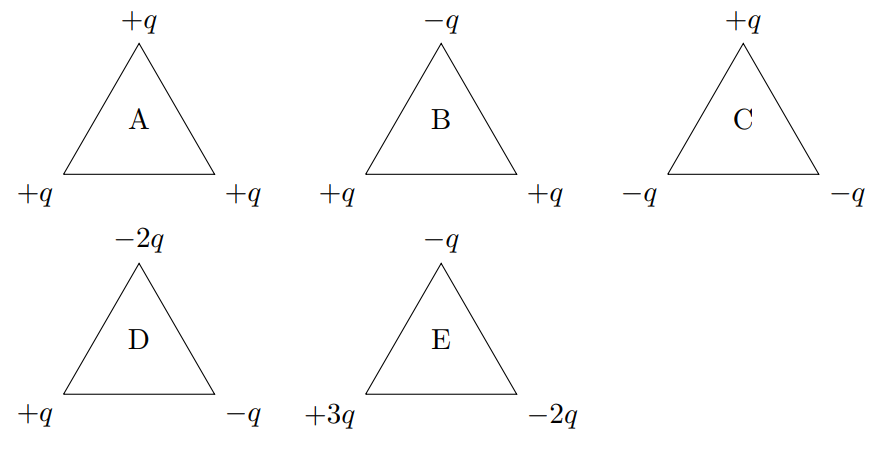
\includegraphics{Figures/Figure24}

%%%%%%%%%%%%%%%%%%%%%%%%%%%%%%%%%%
%%%%%%%%%%%%%%%%%%%%%%%%%%%%%%%%%%
%%%%%%%%%%%%%%%%%%%%%%%%%%%%%%%%%%

\begin{question}
(AP) The electric field at the center is zero at..

\begin{multicols}{5}
\begin{enumerate}[label=(\alph*)]
    \item A
    \item B
    \item C
    \item D
    \item E
\end{enumerate}
\end{multicols}

\end{question}

\begin{solution}
A (Hint: Don't overthink it! Use common sense if you have any)
\end{solution}

%%%%%%%%%%%%%%%%%%%%%%%%%%%%%%%%%%
%%%%%%%%%%%%%%%%%%%%%%%%%%%%%%%%%%
%%%%%%%%%%%%%%%%%%%%%%%%%%%%%%%%%%

\begin{question}
(AP) The electric field at the center is zero at..

\begin{multicols}{5}
\begin{enumerate}[label=(\alph*)]
    \item A
    \item B
    \item C
    \item D
    \item E
\end{enumerate}
\end{multicols}

\end{question}

\begin{solution}
C (Hint: Make use of superposition, and remember which way the electric field points!)
\end{solution}

%%%%%%%%%%%%%%%%%%%%%%%%%%%%%%%%%%
%%%%%%%%%%%%%%%%%%%%%%%%%%%%%%%%%%
%%%%%%%%%%%%%%%%%%%%%%%%%%%%%%%%%%

\begin{question}
The electric potential at the center is zero at...
\begin{multicols}{5}
\begin{enumerate}[label=(\alph*)]
    \item A
    \item B
    \item C
    \item D
    \item E
\end{enumerate}
\end{multicols}

\end{question}

\begin{solution}
E (Hint: Potential is a scaler!)
\end{solution}

%%%%%%%%%%%%%%%%%%%%%%%%%%%%%%%%%%
%%%%%%%%%%%%%%%%%%%%%%%%%%%%%%%%%%
%%%%%%%%%%%%%%%%%%%%%%%%%%%%%%%%%%

\begin{question}
(AP) From the electric field vector at a point, one can determine which of the following at that point?

\begin{enumerate}
    \item The direction of the electrostatic force on a test charge of known sign
    \item The magnitude of the electrostatic force exerted per unit charge on a test charge
    \item The electrostatic charge
\end{enumerate}

\begin{multicols}{5}
\begin{enumerate}[label=(\alph*)]
    \item I
    \item III 
    \item I \& II
    \item II \& III
    \item All 3
\end{enumerate}
\end{multicols}

\end{question}

\begin{solution}
C (Hint: Review what an electric field is!)
\end{solution}

%%%%%%%%%%%%%%%%%%%%%%%%%%%%%%%%%%
%%%%%%%%%%%%%%%%%%%%%%%%%%%%%%%%%%
%%%%%%%%%%%%%%%%%%%%%%%%%%%%%%%%%%

\begin{question}
(AP) A circular ring made of an insulating material is cut in half.  One half is given a charge -q uniformly distributed along its arc.  The other half is given a charge +q also uniformly distributed along its arc.  The two halves are then rejoined with insulation at the junctions J, as shown above.  If there is no change in the charge distributions, what is the direction of the net electrostatic force on an electron located at the center of the circle? 
\begin{enumerate}[label=(\alph*)]
    \item Toward the top of the page
    \item Toward the bottom of the page
    \item To the right
    \item To the left
    \item Into the page
\end{enumerate}

\end{question}

\begin{solution}
B (Hint: Draw it out!)
\end{solution}

%%%%%%%%%%%%%%%%%%%%%%%%%%%%%%%%%%
%%%%%%%%%%%%%%%%%%%%%%%%%%%%%%%%%%
%%%%%%%%%%%%%%%%%%%%%%%%%%%%%%%%%%

\begin{question}
(AP) Two metal spheres are initially uncharged are mounted on insulating stands. A negatively charged rubber rod is brought close to, but does not make contact with, sphere X. Sphere Y is then brought close to X on the side opposite to the rod. Y is allowed to touch X and then is removed far away. The rubber rod is then moved far away from X and Y. What are the final charges on the spheres?

\begin{center}
\begin{tabular}{ |c|c|c| } 
 \hline
       & Sphere X & Sphere Y \\ 
 A      & Zero  & Zero  \\ 
 B      & Negative  & Negative  \\ 
 C      & Negative  & Positive  \\ 
 D      & Positive  & Negative  \\ 
 E      & Positive  & Positive  \\ 

 \hline
\end{tabular}
\end{center}

\end{question}

\begin{solution}
D (Hint: Draw it out. Protons can't move!)
\end{solution}

%%%%%%%%%%%%%%%%%%%%%%%%%%%%%%%%%%
%%%%%%%%%%%%%%%%%%%%%%%%%%%%%%%%%%
%%%%%%%%%%%%%%%%%%%%%%%%%%%%%%%%%%

\begin{question}
(AP) Two initially uncharged conductors, 1 and 2, are mounted on insulating stands and are in contact. A negatively charged rod is brought near conductor 1, at the opposite side of conductor 2, but does not touch them. With the rod held in place, conductor 2 is moved to the right by pushing its stand, so the conductors are separated. Which of the following is now true about the charge of conductor 2?
\begin{multicols}{5}
\begin{enumerate}[label=(\alph*)]
    \item no charge
    \item positive
    \item negative
    \item unknown
    \item no change
\end{enumerate}
\end{multicols}

\end{question}

\begin{solution}
E (Hint: Potential is a scaler!)
\end{solution}

%%%%%%%%%%%%%%%%%%%%%%%%%%%%%%%%%%
%%%%%%%%%%%%%%%%%%%%%%%%%%%%%%%%%%
%%%%%%%%%%%%%%%%%%%%%%%%%%%%%%%%%%
\newpage
As shown below, two particles, each of charge +Q, are fixed at opposite corners of a square that lies in the plane of the page. A positive test charge +q is placed at a third corner. Use this information for the next two questions.

\begin{center}
% \begin{tikzpicture}
% \draw (0,0) -- (0,2) -- (2,2) -- (2,0) -- (0,0);
% \node[above right] at (0,0) {$+q$};
% \node[below right] at (0,2) {$+Q$};
% \node[above left] at (2,0) {$+Q$};
% \end{tikzpicture}
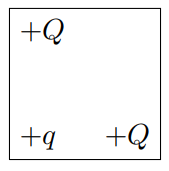
\includegraphics{Figures/Figure25}
\end{center}

%%%%%%%%%%%%%%%%%%%%%%%%%%%%%%%%%%
%%%%%%%%%%%%%%%%%%%%%%%%%%%%%%%%%%
%%%%%%%%%%%%%%%%%%%%%%%%%%%%%%%%%%

\begin{question}
(AP) What is the direction of the force on the test charge due to the two other charges?

\begin{enumerate}[label=(\alph*)]
    \item top right
    \item right
    \item bottom right
    \item down
    \item bottom left
\end{enumerate}

\end{question}

\begin{solution}
E (Hint: Look at the force exerted by each individual particle first)
\end{solution}

%%%%%%%%%%%%%%%%%%%%%%%%%%%%%%%%%%
%%%%%%%%%%%%%%%%%%%%%%%%%%%%%%%%%%
%%%%%%%%%%%%%%%%%%%%%%%%%%%%%%%%%%

\begin{question}
(AP) If F is the magnitude of the force on the test charge due to only one of the other charges, what is the magnitude of the net force acting on the test charge due to both of these charges?
\begin{multicols}{5}
\begin{enumerate}[label=(\alph*)]
    \item Zero
    \item $\frac{F}{\sqrt{2}}$
    \item F
    \item $\sqrt{2}$F
    \item 2
\end{enumerate}
\end{multicols}

\end{question}

\begin{solution}
D (Hint: Why isn't it 2F? First calculate vector form, then convert to magnitude)
\end{solution}


%%%%%%%%%%%%%%%%%%%%%%%%%%%%%%%%%%
%%%%%%%%%%%%%%%%%%%%%%%%%%%%%%%%%%
%%%%%%%%%%%%%%%%%%%%%%%%%%%%%%%%%%

\begin{question}
(AP) If the only force acting on an electron is due to a uniform electric field, the electron moves with constant
\begin{enumerate}[label=(\alph*)]
    \item acceleration in a direction opposite to that of the field
    \item acceleration in the direction of the field
    \item acceleration in a direction perpendicular to that of the field
    \item speed in a direction opposite to that of the field
    \item speed in the direction of the field
\end{enumerate}

\end{question}

\begin{solution}
A (Hint: Which ways to field lines point again?)
\end{solution}

%%%%%%%%%%%%%%%%%%%%%%%%%%%%%%%%%%
%%%%%%%%%%%%%%%%%%%%%%%%%%%%%%%%%%
%%%%%%%%%%%%%%%%%%%%%%%%%%%%%%%%%%
\newpage
Particle of charge Q is located at (-2,0) and another particle of charge -4Q is located at (2,0). Assume the particles are isolated from all other charges. P is a point on the y axis above the x axis. Use this information to answer the next two questions:

%%%%%%%%%%%%%%%%%%%%%%%%%%%%%%%%%%
%%%%%%%%%%%%%%%%%%%%%%%%%%%%%%%%%%
%%%%%%%%%%%%%%%%%%%%%%%%%%%%%%%%%%
\begin{question}
(AP) Which of the following describes the direction of the electric field at point P
\begin{multicols}{5}
\begin{enumerate}[label=(\alph*)]
    \item +x
    \item +y
    \item -y
    \item -x and +y
    \item +x and -y
\end{enumerate}
\end{multicols}

\end{question}

\begin{solution}
E (Hint: Draw your electric field lines! Remember the charges aren't equal.)
\end{solution}

%%%%%%%%%%%%%%%%%%%%%%%%%%%%%%%%%%
%%%%%%%%%%%%%%%%%%%%%%%%%%%%%%%%%%
%%%%%%%%%%%%%%%%%%%%%%%%%%%%%%%%%%

\begin{question}
(AP) At which of the following points on the x-axis is the electric field zero?
\begin{multicols}{5}
\begin{enumerate}[label=(\alph*)]
    \item (-6,0)
    \item (-3,0)
    \item (-1,0)
    \item (1,0)
    \item (6,0)
\end{enumerate}
\end{multicols}

\end{question}

\begin{solution}
A (Hint: Draw MOARRR lines! Or superimpose the electric field equation. Your choice.)
\end{solution}

%%%%%%%%%%%%%%%%%%%%%%%%%%%%%%%%%%
%%%%%%%%%%%%%%%%%%%%%%%%%%%%%%%%%%
%%%%%%%%%%%%%%%%%%%%%%%%%%%%%%%%%%

\begin{question}
(AP) When a negatively charged rod is brought near, but does not touch, an initially uncharged electroscope, the leaves spring apart. (I) When the electroscope is then touched with a finger, the leaves collapse. When the finger and finally the rod are removed, the leaves spring apart a second time (II). The charge on the leaves is:
\begin{enumerate}[label=(\alph*)]
    \item positive in both I and II
    \item negative in I and III
    \item positive in I, negative in III
    \item negative in I, positive in III
    \item impossible to determine in either I or III
\end{enumerate}

\end{question}

\begin{solution}
E (Hint: Draw it out! It's first charging by separation then charging by induction)
\end{solution}

%%%%%%%%%%%%%%%%%%%%%%%%%%%%%%%%%%
%%%%%%%%%%%%%%%%%%%%%%%%%%%%%%%%%%
%%%%%%%%%%%%%%%%%%%%%%%%%%%%%%%%%%
\newpage
\begin{question}
Two experiments are performed using a pair of solid metal spheres connected by a switch. Both spheres are grounded before each experiment so that they initially have no charge.

\emph{Experiment I:} A positively charged rod is brought near sphere A while the the switch is closed, the switch is opened, and the rod is then removed.

\emph{Experiment II:} A positively charged rod is touched to sphere A while the switch is closed, the switch is opened, and the rod is then removed.

Which of the following describes the charge on the spheres after both experiments?
\begin{enumerate}[label=(\alph*)]
    \item After I: both have no charge; After II: both are positive
    \item After I: A is negative and B is positive; After II: A is positive and B is negative
    \item After I: A is negative and B is positive; After II: both are positive
    \item After I and II: both are positive
    \item After I and II: A is positive and B is negative
\end{enumerate}

\end{question}

\begin{solution}
C (Hint: There's a lot going on. Draw lots of diagrams, and use a process of elmination!)
\end{solution}

%%%%%%%%%%%%%%%%%%%%%%%%%%%%%%%%%%
%%%%%%%%%%%%%%%%%%%%%%%%%%%%%%%%%%
%%%%%%%%%%%%%%%%%%%%%%%%%%%%%%%%%%
%%%%%%%%%%%%%%%%%%%%%%%%%%%%%%%%%%
%%%%%%%%%%%%%%%%%%%%%%%%%%%%%%%%%%
%%%%%%%%%%%%%%%%%%%%%%%%%%%%%%%%%%
%%%%%%%%%%%%%%%%%%%%%%%%%%%%%%%%%%
%%%%%%%%%%%%%%%%%%%%%%%%%%%%%%%%%%
%%%%%%%%%%%%%%%%%%%%%%%%%%%%%%%%%%
%%%%%%%%%%%%%%%%%%%%%%%%%%%%%%%%%%
%%%%%%%%%%%%%%%%%%%%%%%%%%%%%%%%%%
%%%%%%%%%%%%%%%%%%%%%%%%%%%%%%%%%%
%%%%%%%%%%%%%%%%%%%%%%%%%%%%%%%%%%
%%%%%%%%%%%%%%%%%%%%%%%%%%%%%%%%%%
%%%%%%%%%%%%%%%%%%%%%%%%%%%%%%%%%%

\newpage
\section{Solutions}


\printsolutions

\newpage
\section{Solutions}
\printsolutions[chapter]

\newpage
\section{Solutions}
\printsolutions[chapter]

\end{document}